\section{Einleitung}
In der Durchführung der globalen Energiewende spielt die Windkraft eine große Rolle. Jedoch treffen Projekte zum Bau großer Anlagen immer wieder auf Widerstand der Anwohner aufgrund der Verunstaltung der Landschaft. Das SAILWIND Projekt soll dem entgegen kommen und entstand aus der Motivation heraus, kleine, griechische Segelwindmühlen, zu renovieren. 
\begin{figure}[H]
	\centering
	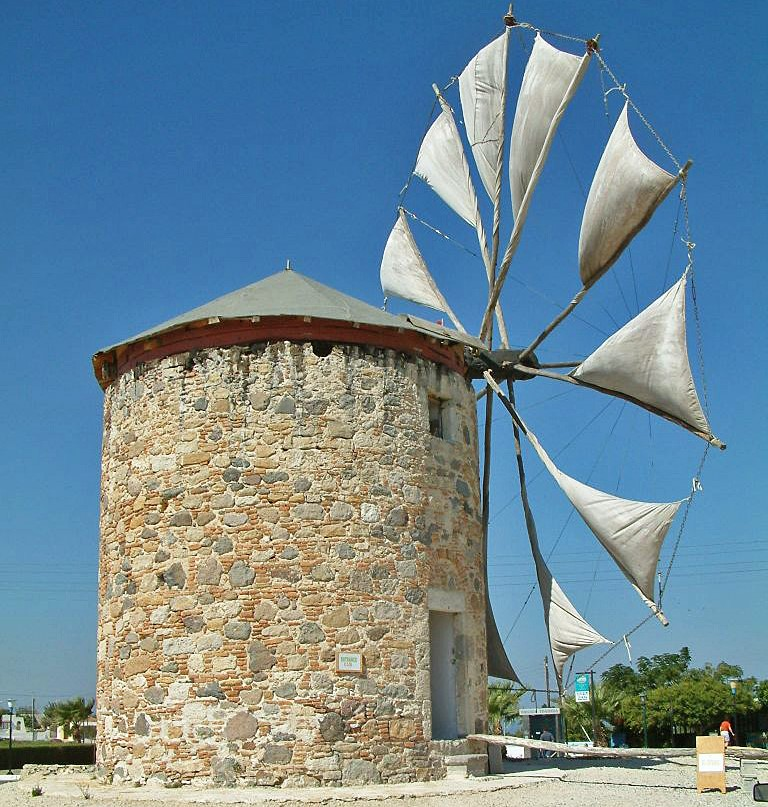
\includegraphics[width=0.6\linewidth]{images/Sailwind/greekSailWindMill.jpg}
	\caption[Segelwindmühle auf der griechischen Insel Kos]{Segelwindmühle auf der griechischen Insel Kos \protect\cite{windMill}}
	\label{fig:sailWindMill}
\end{figure}
\noindent
Vor 3000 Jahren dienten diese noch zum Antrieb von Wasserrädern für den Getreidebau. Mit der Umsetzung des Projekts sollen nun zahlreiche dieser heute ungenutzten Bauwerke zur Erzeugung erneuerbarer Energie umfunktioniert werden. Dabei soll die Optik der Mühlen äußerlich möglichst unverändert bleiben. Lediglich die Segel werden erneuert und die Welle an einen Generator gekoppelt, der bei einer Windstärke von 14 m/s eine Spitzenleistung von 5 kW abgeben soll. Diese reicht aus, um z.B. ein ganzes Restaurant zu versorgen. \cite{industrProjektSailwind} Um die Windmühle effizient zu betreiben, soll eine voll automatisierte Steuerung integriert werden, welche die Segel der Windstärke und -Richtung entsprechend einstellt. Die Einstellung der Segel geschieht dabei über die Verbindung einer Seilführung (wie in \autoref{fig:sailWindMill} zu sehen) mit einer motorisierten Linearführung.
\subsection{Ausgangssituation}
Die vorliegende Arbeit beruht auf den Erkenntnissen einer Gruppe von Studenten, die bereits einen Versuch unternahmen, einen maßstabsgetreuen Prototypen einer automatisierten Segelwindmühle zu entwickeln. Für die Umsetzung des Projekts konnte die Firma Igus als Sponsor gewonnen werden, die neben einem Betrag von 10.000 Euro wichtige Bauteile für den Bau der Windmühle, darunter die Linearführung, zur Verfügung stellt. Die Gruppe befasste sich zunächst mit der Entwicklung einer Logikeinheit zur Berechnung der optimalen Segelstellung für die maximale Ausgangsleistung aufgrund der Windbedingungen und anschließend mit dem Entwurf einer Steuerplatine. Zusätzlich musste die Kommunikation zwischen diesen beiden Systemen realisiert werden. Es stellte sich heraus, dass die Umsetzung des Logikteils weitreichende Untersuchungen und Anwendung komplexer Methoden erfordert. Mit Beendigung des Projekts wurde dazu zwar eine Lösung präsentiert werden, jedoch konnte die Steuerplatine aus zeitlichen Gründen nicht mehr fertiggestellt werden. 
\subsection{Ziel}
Da sich die Aufgabenstellung der vorhergegangenen Gruppe im Rahmen des Bachelorprojekts als zu umfangreich erwies, konzentriert sich diese Arbeit auf die Neuentwicklung der Steuerplatine inklusive Implementierung der Firmware. Das System soll über eine Ethernet-Verbindung die Logikeinheit mit allen relevanten Daten versorgen, sowie umgekehrt Befehle zur Anpassung der Segelstellung empfangen und durch Ansteuerung der Linearführung umsetzen. Die Entwicklung und auch die Wiederverwendung der Logikeinheit ist nicht Teil der Arbeit, es soll lediglich eine Kommunikationsschnittstelle vorbereitet werden.
\newpage



